%% LyX 2.2.2 created this file.  For more info, see http://www.lyx.org/.
%% Do not edit unless you really know what you are doing.
\documentclass[english]{article}
\usepackage[T1]{fontenc}
\usepackage[latin9]{inputenc}
\usepackage{float}
\usepackage{graphicx}
\usepackage{babel}
\begin{document}

\part{ELECTRONICA III EJERCICIO 7}

\section{Contadores}

El hecho de que el flip flop presente una entrada de clock que habilite
un cambio de estado a la salida, permite que se puedan implementar
los flip flops para contar una cantidad de ciclos de clocks que han
transcurrido en el tiempo. Este dispositivo que permite construir
la implementaci�n con flip flops es llamado contador, y existen dos
tipos los cuales son: contador asincr�nico y contador sincr�nico.
A continuaci�n se presenta una implementaci�n de flip flops tipo ``T''
para el contador asincr�nico y para el contador sincr�nico:

\begin{figure}[H]
\begin{centering}
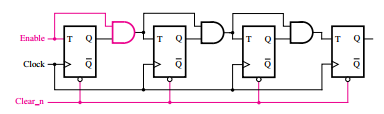
\includegraphics[scale=0.4]{sincCOUNTER.PNG}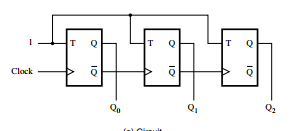
\includegraphics[scale=0.4]{asincCOUNTER.PNG}
\par\end{centering}
\caption{Contador Sincr�nico y Asincr�nico}

\end{figure}

Como se puede ver en el dise�o del contador sincr�nico (imagen de
la izquierda) los flip flops habilitan el cambio de estado al mismo
tiempo (la entrada de clock es la misma para todos, clock sincr�nico),
mientras que para el contador asincr�nico la entrada de clock de los
flip flops proviene del flip flop anterior. Esto �ltimo provoca en
los contadores asincr�nicos una dependencia mayor del delay de los
flip flops en su funcionamiento.

\subsection{Implementaci�n}

En esta parte del art�culo se propone implementar un contador de 3
bits (uno asincr�nico y otro sincr�nico) e intentar medir su m�xima
velocidad de operaci�n. El dise�o a utilizar es el mismo que el presentado
en la imagen anterior (con solo tres flip flops, uno por bit) pero
con flip flops tipo D. Para lograr esto se propuso el siguiente dise�o
para lograr un flip flop tipo T a partir de uno tipo D y as� poder
realizar los contadores:

\begin{figure}[H]
\begin{centering}
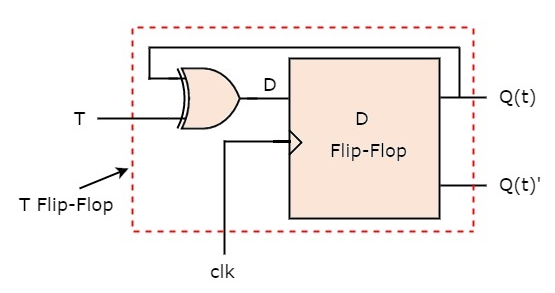
\includegraphics[scale=0.4]{TflipflopWithD.PNG}
\par\end{centering}
\caption{Flip Flop tipo T a partir del tipo D}

\end{figure}


\subsection{M�xima Velocidad de Operaci�n}

Para lograr estimar la m�xima velocidad de operaci�n, se aument� la
frecuencia del clock hasta que esta sea lo suficientemente elevada
para que los flip flops no puedan seguir el conteo correctamente.
Lo que se obtuvo fue que el contador asincr�nico ceso de operar correctamente
a una frecuencia de clock de $21MHz$ mientras que el contador sincr�onico
lo hizo a una frecuencia de clock de $45MHz$.

Esto tiene sentido, ya que seg�n la datasheet de los flip flops utilizados
el tiempo de propagaci�n es del orden de los $20ns$. Esto quiere
decir que a una frecuencia $f=\frac{1}{20ns}=50MHz$ es esperable
que el contador no actualize la cuenta a tiempo. Esto es para el flip
flop sincr�nico, pero para el asincr�nico el tiempo de progragaci�n
se multiplica por la cantidad de bits del contador, o lo que es lo
mismo, por la cantidad de flip flops. Para el caso del contador de
tres bits, la frecuencia de operaci�n se reduce a un tercio de la
que se ten�a para el contador sincr�nico.

Vale aclarar que lo estimado te�ricamente con los par�metros de la
hoja de datos y lo medido no se ajusta perfectamente, pero esto es
esperable debido a las dificultades de medir con el osciloscopio en
altas frecuencias de trabajo y adem�s porque no solo existen flip
flops en el circuito, si no que se han utilizado otras compuertas
como las AND y las XOR que no se han incorporado en el an�lisis. De
todas maneras, se puede notar que el contador sincr�nico permite aumentar
m�s la frecuencia de trabajo (con respecto al contador asincr�nico)
sin que se afecte el funcionamiento.
\end{document}
